\part{软件}
\setcounter{section}{0}
\section{压缩刻录}
\subsection{unetbootin-制作usb启动盘}
准备工作
\begin{itemize}
\item u盘
\item iso镜像文件--\href{http://releases.ubuntu.com/precise/}{ubuntu-12.04.2-desktop-amd64.iso}
\item 刻录软件--\href{http://www.oschina.net/news/9166/oschina-os-week-recommended-UNetbootin}{unetbootin-linux-583}
\end{itemize} 

操作步骤
\begin{enumerate}
\item 格式化u盘
\begin{itemize}
\item 查看u盘信息
\begin{lstlisting}[style=BASH]
hjy@jy:~$ mount
/dev/sdb1 on /media/KINGSTON type vfat (rw,nosuid,nodev,uid=1000,gid=1000,shortname=mixed,dmask=0077,utf8=1,showexec,flush,uhelper=udisks)
\end{lstlisting}

\item 卸载u盘
\begin{lstlisting}[style=BASH]
hjy@jy:~$ umount /media/KINGSTON
\end{lstlisting}

\item 格式化
\begin{lstlisting}[style=BASH]
hjy@jy:~$ mkfs -t vfat /dev/sdb1
\end{lstlisting}
\end{itemize}
\item 启动并设置unetbootin-linux-583参数\\
\begin{figure}[!htbp]
	\centering
	\caption{参数设置}  
		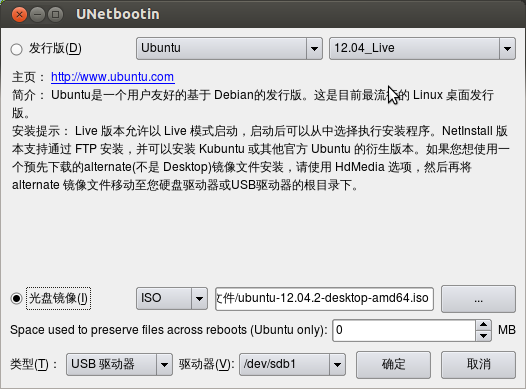
\includegraphics[scale=0.35]{figs/unetbootin_set.png}
    	\label{fig:unetbootin_set}
\end{figure}
注意:\textcolor{red}{软件能够识别u盘--u盘一定要插在电脑上}
\end{enumerate}
\clearpage

\section{聊天工具}
\section{视频软件}
\section{音乐软件}
\section{游戏软件}
\section{网络游戏}
\section{浏览器}
\section{图形图像}
\section{输入法}
\section{下载工具}
\section{办公软件}
\section{阅读翻译}
\section{系统工具}
\section{编程开发}
\section{其他软件}
\section{安全杀毒}















